 % Created 2021-11-03 mié 11:39
% Intended LaTeX compiler: lualatex
\documentclass[table]{scrartcl}
\usepackage[left=1.5cm,right=1.5cm,bottom=3cm,top=2.5cm,letterpaper]{geometry}
\usepackage[spanish, es-nodecimaldot, es-tabla]{babel}
\usepackage[utf8]{inputenc}
\usepackage{blindtext}
\usepackage{multicol}
\usepackage{subfigure}
\usepackage[most]{tcolorbox}
\usepackage{etoolbox}
\usepackage{minted}
\usepackage{hyperref}
% \usepackage[table,xcdraw]{xcolor}
\usepackage{longtable}
\usepackage{multirow}
\usepackage[default]{comfortaa}
\usepackage[T1]{fontenc}
\usepackage{float}
\usepackage{caption}
\usepackage{breqn}
\usemintedstyle{emacs}
\usepackage[ruled,vlined]{algorithm2e}
\newenvironment{code}{\captionsetup{type=listing}}{}
\definecolor{custom}{HTML}{F0F0F0}
\setminted{frame=single,xleftmargin=1cm,breaklines=true,bgcolor=custom,fontsize=\scriptsize,linenos}
\renewcommand\listoflistingscaption{Índice de \listingscaption\@s}
\renewcommand{\listingscaption}{Código}
\BeforeBeginEnvironment{listing}{\begin{code}}
  \AfterEndEnvironment{listing}{\end{code}}
\BeforeBeginEnvironment{minted}{\begin{code}}
  \AfterEndEnvironment{minted}{\end{code}}
\author{Monsalvo Bolaños Melissa Monserrat y Romero Andrade Cristian}
\date{\today}
\title{Practica 6}
\hypersetup{
  pdfauthor={Monsalvo Bolaños Melissa Monserrat y Romero Andrade Cristian},
  pdftitle={Practica 6},
  pdfkeywords={},
  pdfsubject={},
  pdfcreator={Emacs 27.2 (Org mode 9.6)},
  pdflang={English}}

\newcommand{\tituloTrabajo}{Práctica No 6\\Secuenciador básico}
% \newcommand{\fechaEntrega}{21 de octubre de 2021}

\usepackage{subfiles}
\usepackage[backend=biber,style=apa]{biblatex}
\addbibresource{../bib.bib}

\begin{document}
\begin{titlepage}
  \centering

    {\scshape{\Huge Facultad de Ingeniería\par{}}}\vspace{0.25cm}

    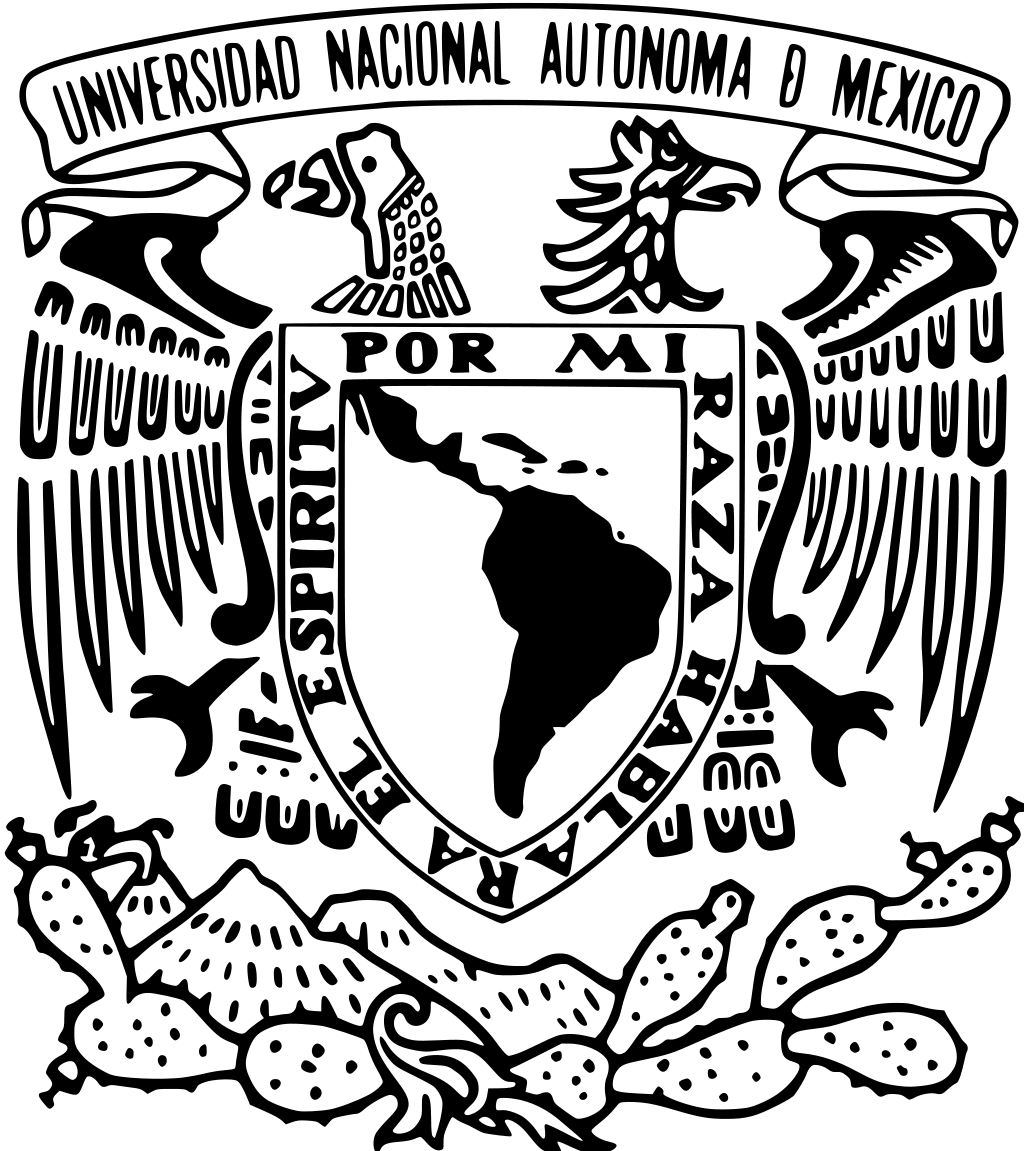
\includegraphics[width=0.25\textwidth]{../img_common/unam_logo}\vspace{0.5cm}

    {\scshape{\Large Lab. Organización y Arquitectura de Computadoras\par{}}}\vfill{}


    {\huge \textbf{\tituloTrabajo{}}}\vfill{}


    {\Large
      Alumnos
      \begin{itemize}

        \item Monsalvo Bolaños Melissa Monserrat

        \item Romero Andrade Cristian
      \end{itemize}
    }\vfill{}

      {\large Grupo: 01\par{}}\vfill{}

    {\large Profesor\\Ing.~Adrian Ulises Mercado Martinez}\vfill{}
    \vfil{}
    {\large Semestre\\\textbf{2022--1}}
    \vfill{}
    % {\large Fecha de Entrega\\\fechaEntrega}
    % \vfill{}
    
\includegraphics[width=0.1\textwidth]{../img_common/inge_logo}

\end{titlepage}

\date{}
\tableofcontents{}

\section{Objetivo}
\label{sec:objetivo}
Familiarizar al alumno en el conocimiento del secuenciador básico, el cual es
una parte fundamental del procesador.

\section{Introducción}\label{sec:introduccion}
Para el diseño de los módulos de control de una computadora se requieren máquinas de
estados que sean capaces de ejecutar algoritmos más complejos. Haciendo modificaciones
y agregando componentes a la variante del direccionamiento implícito se pueden crear
máquinas de estados que efectúen cartas ASM con llamadas a subrutinas, estructuras DO
WHILE, iteraciones tipo FOR, entre otras. Los dispositivos que son capaces de efectuar este
tipo de operaciones son llamados secuenciadores.

A continuación, se muestra el diagrama de bloques de un secuenciador básico. Como puede
observar en el diagrama, la dirección del estado siguiente, dada por el bus $Y$, puede venir de
dos lugares posibles: Del registro $\mu{}PC$ o de la entrada $D$.
\begin{figure}[H]
  \centering
  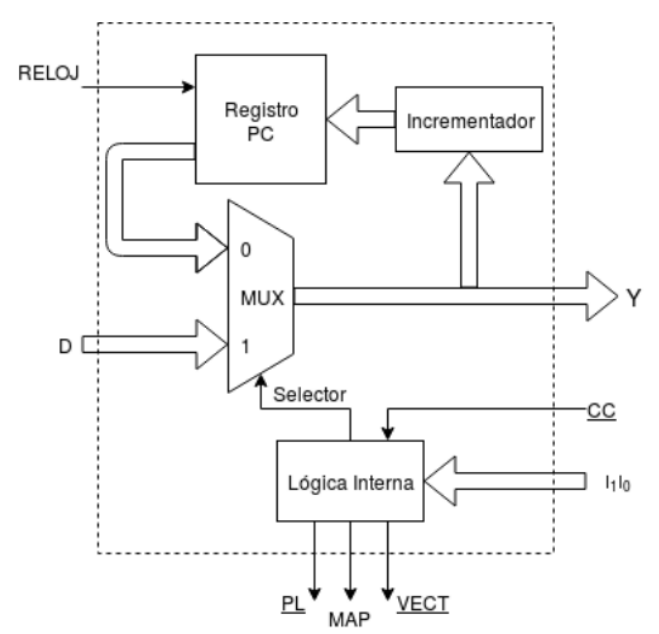
\includegraphics[width=0.4\textwidth]{./img/1}
  \caption{Diagrama de bloques interno de un secuenciador básico}\label{fig:1}
\end{figure}

El secuenciador cuenta con una lógica interna que se encarga de generar las señales que
controlan al multiplexor. Dependiendo de la instrucción dada por las líneas $I_1$ e $I_0$ y de la línea
$\underline{CC}$, la lógica es capaz de seleccionar entre la salida del registro $\mu{}PC$ o la
entrada $D$.

La lógica interna también genera las líneas $\underline{PL}$, $\underline{MAP}$
y $\underline{VECT}$, las cuales seleccionan unos registros cuyas salidas están
conectadas a la entrada $D$ del secuenciador. De esta forma la dirección de salto
puede venir de tres lugares distintos.
\begin{figure}[H]
  \centering
  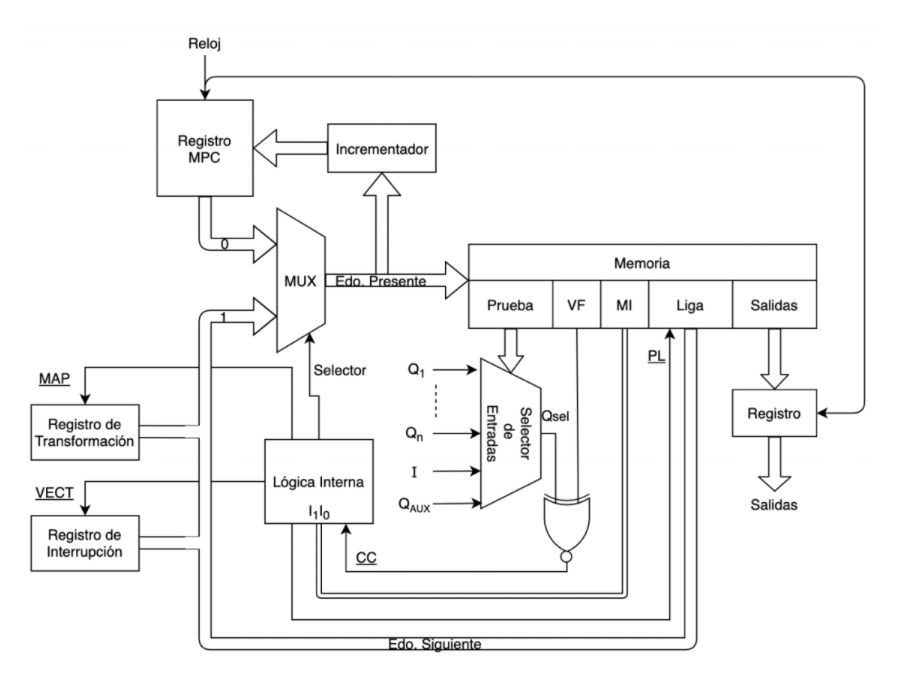
\includegraphics[width=0.7\textwidth]{./img/dia_fin_ex}
  \caption{Diagrama de bloques interno de un secuenciador básico conectado a memoria}\label{fig:dia_fin_ex}
\end{figure}

\subsection{Paso Contiguo (C) [00]}\label{sec:paso-contiguo-c}
En la instrucción continúa la dirección del estado siguiente la proporciona el
registro $\mu{}PC$.
\begin{figure}[H]
  \centering
  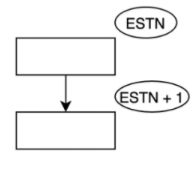
\includegraphics[width=0.2\textwidth]{./img/pc}
  \caption{Carta ASM de Paso contiguo}\label{fig:pc}
\end{figure}

\subsection{Salto Condicional (SC) [01]}\label{sec:salto-cond-sc}
En esta instrucción se revisa el valor de la línea $\underline{CC}$, si es igual a uno, la dirección del estado
siguiente la proporciona el registro $\mu{}PC$; si es igual a cero, la dirección del estado siguiente,
contenida en el registro seleccionado por $\underline{PL}$, ingresa a través de la entrada $D$.
\begin{figure}[H]
  \centering
  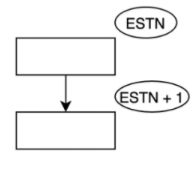
\includegraphics[width=0.2\textwidth]{./img/pc}
  \caption{Carta ASM de Salto Condicional}\label{fig:sc}
\end{figure}

\subsection{Salto de Tranformación (ST) [10]}\label{sec:salto-de-tranf}
La dirección del estado siguiente se obtiene del registro seleccionado por la línea de $\underline{MAP}$.
Este registro también está conectado a la entrada D. Aquí se introduce una nueva notación
de carta ASM: un rombo con varias bifurcaciones. La bifurcación que se elija dependerá del
contenido del registro seleccionado por $\underline{MAP}$.
\begin{figure}[H]
  \centering
  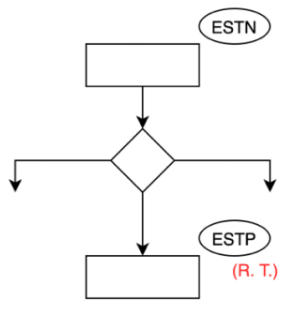
\includegraphics[width=0.2\textwidth]{./img/st}
  \caption{Carta ASM de Salto de Transformación}\label{fig:st}
\end{figure}

\subsection{Salto de Interrupción (SI) [11]}\label{sec:salto-de-interr}
En esta instrucción se revisa el valor de $\underline{CC}$, si es igual a uno, la dirección del estado siguiente
proviene del registro $\mu{}PC$; si es igual a cero, la dirección del estado siguiente, contenida en
el registro seleccionado por $\underline{VECT}$, ingresa a través de la entrada $D$.
\begin{figure}[H]
  \centering
  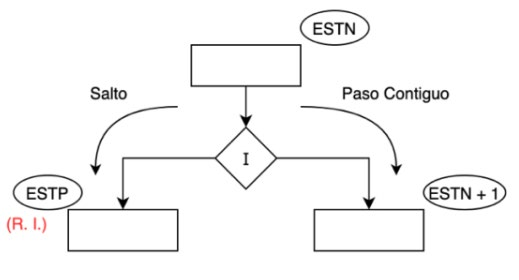
\includegraphics[width=0.4\textwidth]{./img/si}
  \caption{Carta ASM de Salto de Interrupción}\label{fig:si}
\end{figure}




\newpage{}
\section{Desarrollo}
\label{sec:desarrollo}

\subsection{Secuenciador}\label{sec:secuenciador}
Primeramente realizamos la tabla del secuenciador basado en la
figura~\ref{fig:1}. en la cual debemos crear la lógica interna la cual
escribimos la tabla~\ref{tab:sec} de las microinstrucciónes en el siguiente bloque en
\texttt{VHDL}. Donde después creamos el  multiplexor que selecciona la secuencia
si esta es contigua, usando el incrementador (código~\ref{src:mux_sec}) o la que nos
manda la memoria (código~\ref{src:memoria}) ya sea por transferencia o
por interrupción. Nos auxiliamos con otro bloque de
incrementador (código~\ref{src:incrementador}) y un registro (código~\ref{src:registro}) para pasar los
bits.

\begin{center}
  \scriptsize
  \captionof{table}{Lógica interna (Microinstrucciones)}\label{tab:sec}
  \begin{longtable}{|ccc|cccc|c|}
  \hline
  \multicolumn{3}{|c|}{\textbf{Entradas}} & \multicolumn{4}{c|}{\textbf{Salidas}} &  \\ \hline
  \multicolumn{1}{|c|}{\textbf{I1}} & \multicolumn{1}{c|}{\textbf{I0}} & \textbf{$\underline{CC}$} & \multicolumn{1}{c|}{\textbf{$\underline{PL}$}} & \multicolumn{1}{c|}{\textbf{$\underline{MAP}$}} & \multicolumn{1}{c|}{\textbf{$\underline{VECT}$}} & \textbf{Selector} & \textbf{Y} \\ \hline
  \rowcolor[HTML]{D9D9D9}
  \multicolumn{1}{|c|}{\cellcolor[HTML]{D9D9D9}0} & \multicolumn{1}{c|}{\cellcolor[HTML]{D9D9D9}0} & 0 & \multicolumn{1}{c|}{\cellcolor[HTML]{D9D9D9}1} & \multicolumn{1}{c|}{\cellcolor[HTML]{D9D9D9}1} & \multicolumn{1}{c|}{\cellcolor[HTML]{D9D9D9}1} & 0 & uPC \\ \hline
  \rowcolor[HTML]{D9D9D9}
  \multicolumn{1}{|c|}{\cellcolor[HTML]{D9D9D9}0} & \multicolumn{1}{c|}{\cellcolor[HTML]{D9D9D9}0} & 1 & \multicolumn{1}{c|}{\cellcolor[HTML]{D9D9D9}1} & \multicolumn{1}{c|}{\cellcolor[HTML]{D9D9D9}1} & \multicolumn{1}{c|}{\cellcolor[HTML]{D9D9D9}1} & 0 & uPC \\ \hline
  \multicolumn{1}{|c|}{0} & \multicolumn{1}{c|}{1} & 0 & \multicolumn{1}{c|}{0} & \multicolumn{1}{c|}{1} & \multicolumn{1}{c|}{1} & 0 & uPC \\ \hline
  \multicolumn{1}{|c|}{0} & \multicolumn{1}{c|}{1} & 1 & \multicolumn{1}{c|}{0} & \multicolumn{1}{c|}{1} & \multicolumn{1}{c|}{1} & 1 & D \\ \hline
  \rowcolor[HTML]{D9D9D9}
  \multicolumn{1}{|c|}{\cellcolor[HTML]{D9D9D9}1} & \multicolumn{1}{c|}{\cellcolor[HTML]{D9D9D9}0} & 0 & \multicolumn{1}{c|}{\cellcolor[HTML]{D9D9D9}1} & \multicolumn{1}{c|}{\cellcolor[HTML]{D9D9D9}0} & \multicolumn{1}{c|}{\cellcolor[HTML]{D9D9D9}1} & 1 & D \\ \hline
  \rowcolor[HTML]{D9D9D9}
  \multicolumn{1}{|c|}{\cellcolor[HTML]{D9D9D9}1} & \multicolumn{1}{c|}{\cellcolor[HTML]{D9D9D9}0} & 1 & \multicolumn{1}{c|}{\cellcolor[HTML]{D9D9D9}1} & \multicolumn{1}{c|}{\cellcolor[HTML]{D9D9D9}0} & \multicolumn{1}{c|}{\cellcolor[HTML]{D9D9D9}1} & 1 & D \\ \hline
  \multicolumn{1}{|c|}{1} & \multicolumn{1}{c|}{1} & 0 & \multicolumn{1}{c|}{1} & \multicolumn{1}{c|}{1} & \multicolumn{1}{c|}{0} & 0 & uPC \\ \hline
  \multicolumn{1}{|c|}{1} & \multicolumn{1}{c|}{1} & 1 & \multicolumn{1}{c|}{1} & \multicolumn{1}{c|}{1} & \multicolumn{1}{c|}{0} & 1 & D \\ \hline
\end{longtable}

\end{center}

\begin{code}
  \caption{\texttt{logica_interna.vhd}}\label{src:logica_interna}
  \inputminted{vhdl}{./logica_interna.vhd}
\end{code}

\begin{code}
  \caption{\texttt{mux_sec.vhd}}\label{src:mux_sec}
  \inputminted{vhdl}{./mux_sec.vhd}
\end{code}

\begin{code}
  \caption{\texttt{incrementador.vhd}}\label{src:incrementador}
  \inputminted{vhdl}{./incrementador.vhd}
\end{code}

\begin{code}
  \caption{\texttt{registro.vhd}}\label{src:registro}
  \inputminted{vhdl}{./registro.vhd}
\end{code}


Después tenemos como resultado (después de conectar cada bloque) el siguiente
diagrama (figura~\ref{fig:dia_sec}).
\begin{figure}[H]
  \centering
  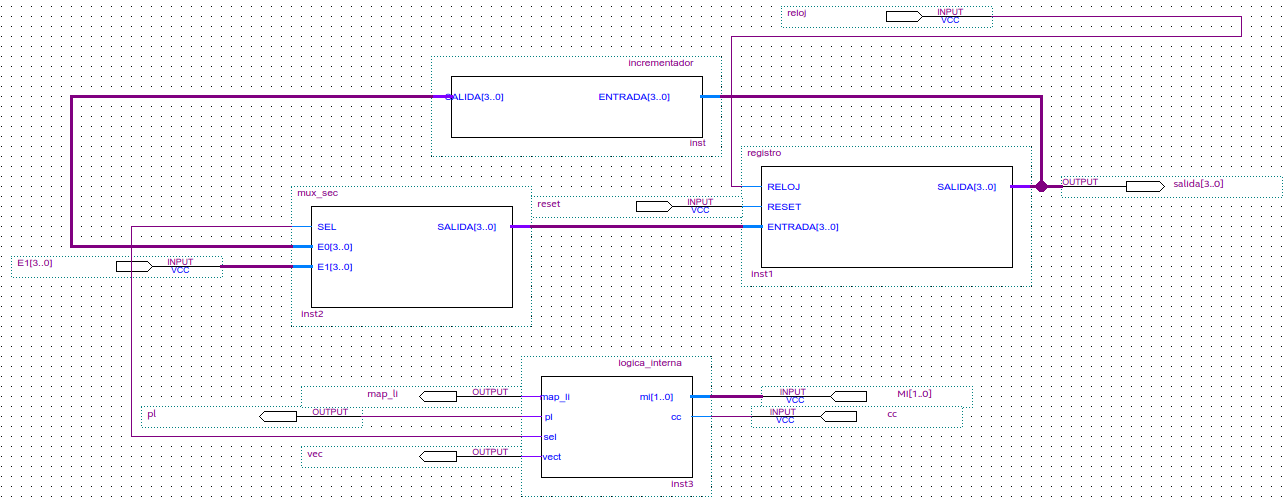
\includegraphics[width=\textwidth]{./img/dia_sec}
  \caption{Diagrama de bloques del secuenciador}\label{fig:dia_sec}
\end{figure}
\newpage{}
\subsection{Carta ASM}\label{sec:carta-asm}
Una vez obtenido el secuenciador, resolvemos la carta ASM objetivo de la practica
(figura~\ref{fig:dia})
\begin{figure}[H]
  \centering
  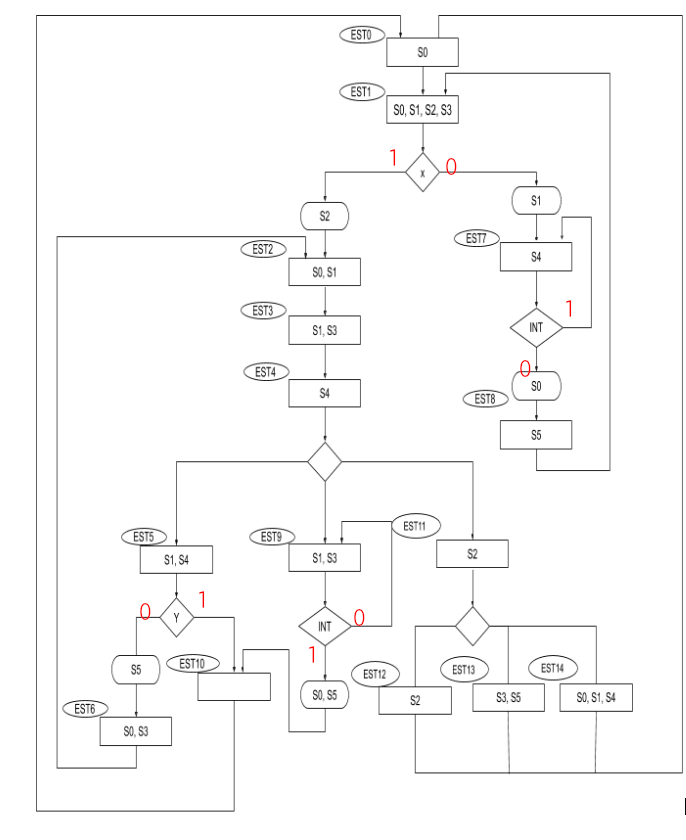
\includegraphics[width=0.53\textwidth]{./img/dia}
  \caption{Carta ASM}\label{fig:dia}
\end{figure}

Definimos las entradas, MI, estados (tabla~\ref{tab:in}) y la tabla de verdad de la carta ASM (tabla~\ref{tab:asm}).
\begin{center}
  \scriptsize
  \captionof{table}{Valores binarios de entradas y MI}\label{tab:in}
  \begin{longtable}{llllllll|lrrrr|}
\cline{9-13}
 &  &  &  &  &  &  &  & \multicolumn{5}{l|}{Estados} \\ \cline{9-13}
 &  &  &  &  &  &  &  & \multicolumn{1}{l|}{\cellcolor[HTML]{D9D9D9}EST0} & \multicolumn{1}{r|}{\cellcolor[HTML]{D9D9D9}0} & \multicolumn{1}{r|}{\cellcolor[HTML]{D9D9D9}0} & \multicolumn{1}{r|}{\cellcolor[HTML]{D9D9D9}0} & \cellcolor[HTML]{D9D9D9}0 \\ \cline{9-13}
 &  &  &  &  &  &  &  & \multicolumn{1}{l|}{EST1} & \multicolumn{1}{r|}{0} & \multicolumn{1}{r|}{0} & \multicolumn{1}{r|}{0} & 1 \\ \cline{9-13}
 &  &  &  &  &  &  &  & \multicolumn{1}{l|}{\cellcolor[HTML]{D9D9D9}EST2} & \multicolumn{1}{r|}{\cellcolor[HTML]{D9D9D9}0} & \multicolumn{1}{r|}{\cellcolor[HTML]{D9D9D9}0} & \multicolumn{1}{r|}{\cellcolor[HTML]{D9D9D9}1} & \cellcolor[HTML]{D9D9D9}0 \\ \cline{9-13}
 &  &  &  &  &  &  &  & \multicolumn{1}{l|}{EST3} & \multicolumn{1}{r|}{0} & \multicolumn{1}{r|}{0} & \multicolumn{1}{r|}{1} & 1 \\ \cline{9-13}
 &  &  &  &  &  &  &  & \multicolumn{1}{l|}{\cellcolor[HTML]{D9D9D9}EST4} & \multicolumn{1}{r|}{\cellcolor[HTML]{D9D9D9}0} & \multicolumn{1}{r|}{\cellcolor[HTML]{D9D9D9}1} & \multicolumn{1}{r|}{\cellcolor[HTML]{D9D9D9}0} & \cellcolor[HTML]{D9D9D9}0 \\ \cline{9-13}
 &  &  &  &  &  &  &  & \multicolumn{1}{l|}{EST5} & \multicolumn{1}{r|}{0} & \multicolumn{1}{r|}{1} & \multicolumn{1}{r|}{0} & 1 \\ \cline{1-3} \cline{5-7} \cline{9-13}
\multicolumn{3}{|l|}{Entrada} & \multicolumn{1}{l|}{} & \multicolumn{3}{l|}{MI} &  & \multicolumn{1}{l|}{\cellcolor[HTML]{D9D9D9}EST6} & \multicolumn{1}{r|}{\cellcolor[HTML]{D9D9D9}0} & \multicolumn{1}{r|}{\cellcolor[HTML]{D9D9D9}1} & \multicolumn{1}{r|}{\cellcolor[HTML]{D9D9D9}1} & \cellcolor[HTML]{D9D9D9}0 \\ \cline{1-3} \cline{5-7} \cline{9-13}
\multicolumn{1}{|r|}{\cellcolor[HTML]{CCCCCC}0} & \multicolumn{1}{r|}{\cellcolor[HTML]{CCCCCC}0} & \multicolumn{1}{l|}{\cellcolor[HTML]{CCCCCC}aux} & \multicolumn{1}{l|}{} & \multicolumn{1}{l|}{\cellcolor[HTML]{D9D9D9}C} & \multicolumn{1}{r|}{\cellcolor[HTML]{D9D9D9}0} & \multicolumn{1}{r|}{\cellcolor[HTML]{D9D9D9}0} &  & \multicolumn{1}{l|}{EST7} & \multicolumn{1}{r|}{0} & \multicolumn{1}{r|}{1} & \multicolumn{1}{r|}{1} & 1 \\ \cline{1-3} \cline{5-7} \cline{9-13}
\multicolumn{1}{|r|}{0} & \multicolumn{1}{r|}{1} & \multicolumn{1}{l|}{X} & \multicolumn{1}{l|}{} & \multicolumn{1}{l|}{SC} & \multicolumn{1}{r|}{0} & \multicolumn{1}{r|}{1} &  & \multicolumn{1}{l|}{\cellcolor[HTML]{D9D9D9}EST8} & \multicolumn{1}{r|}{\cellcolor[HTML]{D9D9D9}1} & \multicolumn{1}{r|}{\cellcolor[HTML]{D9D9D9}0} & \multicolumn{1}{r|}{\cellcolor[HTML]{D9D9D9}0} & \cellcolor[HTML]{D9D9D9}0 \\ \cline{1-3} \cline{5-7} \cline{9-13}
\multicolumn{1}{|r|}{\cellcolor[HTML]{CCCCCC}1} & \multicolumn{1}{r|}{\cellcolor[HTML]{CCCCCC}0} & \multicolumn{1}{l|}{\cellcolor[HTML]{CCCCCC}Y} & \multicolumn{1}{l|}{} & \multicolumn{1}{l|}{\cellcolor[HTML]{D9D9D9}ST} & \multicolumn{1}{r|}{\cellcolor[HTML]{D9D9D9}1} & \multicolumn{1}{r|}{\cellcolor[HTML]{D9D9D9}0} &  & \multicolumn{1}{l|}{EST9} & \multicolumn{1}{r|}{1} & \multicolumn{1}{r|}{0} & \multicolumn{1}{r|}{0} & 1 \\ \cline{1-3} \cline{5-7} \cline{9-13}
\multicolumn{1}{|r|}{1} & \multicolumn{1}{r|}{1} & \multicolumn{1}{l|}{INT} & \multicolumn{1}{l|}{} & \multicolumn{1}{l|}{SI} & \multicolumn{1}{r|}{1} & \multicolumn{1}{r|}{1} &  & \multicolumn{1}{l|}{\cellcolor[HTML]{D9D9D9}EST10} & \multicolumn{1}{r|}{\cellcolor[HTML]{D9D9D9}1} & \multicolumn{1}{r|}{\cellcolor[HTML]{D9D9D9}0} & \multicolumn{1}{r|}{\cellcolor[HTML]{D9D9D9}1} & \cellcolor[HTML]{D9D9D9}0 \\ \cline{1-3} \cline{5-7} \cline{9-13}
 &  &  &  &  &  &  &  & \multicolumn{1}{l|}{EST11} & \multicolumn{1}{r|}{1} & \multicolumn{1}{r|}{0} & \multicolumn{1}{r|}{1} & 1 \\ \cline{9-13}
 &  &  &  &  &  &  &  & \multicolumn{1}{l|}{\cellcolor[HTML]{D9D9D9}EST12} & \multicolumn{1}{r|}{\cellcolor[HTML]{D9D9D9}1} & \multicolumn{1}{r|}{\cellcolor[HTML]{D9D9D9}1} & \multicolumn{1}{r|}{\cellcolor[HTML]{D9D9D9}0} & \cellcolor[HTML]{D9D9D9}0 \\ \cline{9-13}
 &  &  &  &  &  &  &  & \multicolumn{1}{l|}{EST13} & \multicolumn{1}{r|}{1} & \multicolumn{1}{r|}{1} & \multicolumn{1}{r|}{0} & 1 \\ \cline{9-13}
 &  &  &  &  &  &  &  & \multicolumn{1}{l|}{\cellcolor[HTML]{D9D9D9}EST14} & \multicolumn{1}{r|}{\cellcolor[HTML]{D9D9D9}1} & \multicolumn{1}{r|}{\cellcolor[HTML]{D9D9D9}1} & \multicolumn{1}{r|}{\cellcolor[HTML]{D9D9D9}1} & \cellcolor[HTML]{D9D9D9}0 \\ \cline{9-13}

\end{longtable}

\end{center}

\begin{center}
  \tiny
  \captionof{table}{Tabla de verdad}\label{tab:asm}
  \begin{longtable}{|ccc|ccccccccccccccccccc|}
\hline
\rowcolor[HTML]{CC4125}
\multicolumn{3}{|c|}{\cellcolor[HTML]{CC4125}{\color[HTML]{FFFFFF} \textbf{Dirección de memoria}}} & \multicolumn{19}{c|}{\cellcolor[HTML]{CC4125}Contenido de la memoria} \\ \hline
\rowcolor[HTML]{E06666}
\multicolumn{3}{|c|}{\cellcolor[HTML]{E06666}Estado Presente} & \multicolumn{3}{c|}{\cellcolor[HTML]{E06666}} & \multicolumn{3}{c|}{\cellcolor[HTML]{E06666}} & \multicolumn{3}{c|}{\cellcolor[HTML]{E06666}} & \multicolumn{5}{c|}{\cellcolor[HTML]{E06666}Salidas Falsas} & \multicolumn{5}{c|}{\cellcolor[HTML]{E06666}Salidas Verdaderas} \\ \cline{1-3} \cline{13-22}
\rowcolor[HTML]{F6B26B}
\multicolumn{1}{|c|}{\cellcolor[HTML]{F6B26B}Q2} & \multicolumn{1}{c|}{\cellcolor[HTML]{F6B26B}Q1} & Q0 & \multicolumn{3}{c|}{\multirow{-2}{*}{\cellcolor[HTML]{E06666}Prueba}} & \multicolumn{3}{c|}{\multirow{-2}{*}{\cellcolor[HTML]{E06666}Liga Falsa}} & \multicolumn{3}{c|}{\multirow{-2}{*}{\cellcolor[HTML]{E06666}Liga Verdadera}} & \multicolumn{1}{c|}{\cellcolor[HTML]{F6B26B}S5} & \multicolumn{1}{c|}{\cellcolor[HTML]{F6B26B}S3} & \multicolumn{1}{c|}{\cellcolor[HTML]{F6B26B}S2} & \multicolumn{1}{c|}{\cellcolor[HTML]{F6B26B}S1} & \multicolumn{1}{c|}{\cellcolor[HTML]{F6B26B}S0} & \multicolumn{1}{c|}{\cellcolor[HTML]{F6B26B}S5} & \multicolumn{1}{c|}{\cellcolor[HTML]{F6B26B}S3} & \multicolumn{1}{c|}{\cellcolor[HTML]{F6B26B}S2} & \multicolumn{1}{c|}{\cellcolor[HTML]{F6B26B}S1} & S0 \\ \hline
\rowcolor[HTML]{FFE599}
\multicolumn{1}{|c|}{\cellcolor[HTML]{FFE599}0} & \multicolumn{1}{c|}{\cellcolor[HTML]{FFE599}0} & 0 & \multicolumn{1}{c|}{\cellcolor[HTML]{FFE599}1} & \multicolumn{1}{c|}{\cellcolor[HTML]{FFE599}0} & \multicolumn{1}{c|}{\cellcolor[HTML]{FFE599}0} & \multicolumn{1}{c|}{\cellcolor[HTML]{FFE599}0} & \multicolumn{1}{c|}{\cellcolor[HTML]{FFE599}0} & \multicolumn{1}{c|}{\cellcolor[HTML]{FFE599}1} & \multicolumn{1}{c|}{\cellcolor[HTML]{FFE599}0} & \multicolumn{1}{c|}{\cellcolor[HTML]{FFE599}0} & \multicolumn{1}{c|}{\cellcolor[HTML]{FFE599}1} & \multicolumn{1}{c|}{\cellcolor[HTML]{FFE599}0} & \multicolumn{1}{c|}{\cellcolor[HTML]{FFE599}0} & \multicolumn{1}{c|}{\cellcolor[HTML]{FFE599}0} & \multicolumn{1}{c|}{\cellcolor[HTML]{FFE599}0} & \multicolumn{1}{c|}{\cellcolor[HTML]{FFE599}0} & \multicolumn{1}{c|}{\cellcolor[HTML]{FFE599}0} & \multicolumn{1}{c|}{\cellcolor[HTML]{FFE599}0} & \multicolumn{1}{c|}{\cellcolor[HTML]{FFE599}0} & \multicolumn{1}{c|}{\cellcolor[HTML]{FFE599}0} & 0 \\ \hline
\rowcolor[HTML]{B6D7A8}
\multicolumn{1}{|c|}{\cellcolor[HTML]{B6D7A8}0} & \multicolumn{1}{c|}{\cellcolor[HTML]{B6D7A8}0} & 1 & \multicolumn{1}{c|}{\cellcolor[HTML]{B6D7A8}0} & \multicolumn{1}{c|}{\cellcolor[HTML]{B6D7A8}1} & \multicolumn{1}{c|}{\cellcolor[HTML]{B6D7A8}0} & \multicolumn{1}{c|}{\cellcolor[HTML]{B6D7A8}0} & \multicolumn{1}{c|}{\cellcolor[HTML]{B6D7A8}1} & \multicolumn{1}{c|}{\cellcolor[HTML]{B6D7A8}0} & \multicolumn{1}{c|}{\cellcolor[HTML]{B6D7A8}1} & \multicolumn{1}{c|}{\cellcolor[HTML]{B6D7A8}0} & \multicolumn{1}{c|}{\cellcolor[HTML]{B6D7A8}0} & \multicolumn{1}{c|}{\cellcolor[HTML]{B6D7A8}0} & \multicolumn{1}{c|}{\cellcolor[HTML]{B6D7A8}0} & \multicolumn{1}{c|}{\cellcolor[HTML]{B6D7A8}0} & \multicolumn{1}{c|}{\cellcolor[HTML]{B6D7A8}1} & \multicolumn{1}{c|}{\cellcolor[HTML]{B6D7A8}0} & \multicolumn{1}{c|}{\cellcolor[HTML]{B6D7A8}0} & \multicolumn{1}{c|}{\cellcolor[HTML]{B6D7A8}0} & \multicolumn{1}{c|}{\cellcolor[HTML]{B6D7A8}0} & \multicolumn{1}{c|}{\cellcolor[HTML]{B6D7A8}1} & 0 \\ \hline
\rowcolor[HTML]{A2C4C9}
\multicolumn{1}{|c|}{\cellcolor[HTML]{A2C4C9}0} & \multicolumn{1}{c|}{\cellcolor[HTML]{A2C4C9}1} & 0 & \multicolumn{1}{c|}{\cellcolor[HTML]{A2C4C9}1} & \multicolumn{1}{c|}{\cellcolor[HTML]{A2C4C9}0} & \multicolumn{1}{c|}{\cellcolor[HTML]{A2C4C9}0} & \multicolumn{1}{c|}{\cellcolor[HTML]{A2C4C9}0} & \multicolumn{1}{c|}{\cellcolor[HTML]{A2C4C9}1} & \multicolumn{1}{c|}{\cellcolor[HTML]{A2C4C9}1} & \multicolumn{1}{c|}{\cellcolor[HTML]{A2C4C9}0} & \multicolumn{1}{c|}{\cellcolor[HTML]{A2C4C9}1} & \multicolumn{1}{c|}{\cellcolor[HTML]{A2C4C9}1} & \multicolumn{1}{c|}{\cellcolor[HTML]{A2C4C9}0} & \multicolumn{1}{c|}{\cellcolor[HTML]{A2C4C9}0} & \multicolumn{1}{c|}{\cellcolor[HTML]{A2C4C9}0} & \multicolumn{1}{c|}{\cellcolor[HTML]{A2C4C9}0} & \multicolumn{1}{c|}{\cellcolor[HTML]{A2C4C9}0} & \multicolumn{1}{c|}{\cellcolor[HTML]{A2C4C9}0} & \multicolumn{1}{c|}{\cellcolor[HTML]{A2C4C9}0} & \multicolumn{1}{c|}{\cellcolor[HTML]{A2C4C9}0} & \multicolumn{1}{c|}{\cellcolor[HTML]{A2C4C9}0} & 0 \\ \hline
\rowcolor[HTML]{A4C2F4}
\multicolumn{1}{|c|}{\cellcolor[HTML]{A4C2F4}0} & \multicolumn{1}{c|}{\cellcolor[HTML]{A4C2F4}1} & 1 & \multicolumn{1}{c|}{\cellcolor[HTML]{A4C2F4}0} & \multicolumn{1}{c|}{\cellcolor[HTML]{A4C2F4}0} & \multicolumn{1}{c|}{\cellcolor[HTML]{A4C2F4}0} & \multicolumn{1}{c|}{\cellcolor[HTML]{A4C2F4}1} & \multicolumn{1}{c|}{\cellcolor[HTML]{A4C2F4}0} & \multicolumn{1}{c|}{\cellcolor[HTML]{A4C2F4}1} & \multicolumn{1}{c|}{\cellcolor[HTML]{A4C2F4}1} & \multicolumn{1}{c|}{\cellcolor[HTML]{A4C2F4}1} & \multicolumn{1}{c|}{\cellcolor[HTML]{A4C2F4}0} & \multicolumn{1}{c|}{\cellcolor[HTML]{A4C2F4}0} & \multicolumn{1}{c|}{\cellcolor[HTML]{A4C2F4}1} & \multicolumn{1}{c|}{\cellcolor[HTML]{A4C2F4}0} & \multicolumn{1}{c|}{\cellcolor[HTML]{A4C2F4}0} & \multicolumn{1}{c|}{\cellcolor[HTML]{A4C2F4}0} & \multicolumn{1}{c|}{\cellcolor[HTML]{A4C2F4}0} & \multicolumn{1}{c|}{\cellcolor[HTML]{A4C2F4}1} & \multicolumn{1}{c|}{\cellcolor[HTML]{A4C2F4}0} & \multicolumn{1}{c|}{\cellcolor[HTML]{A4C2F4}0} & 0 \\ \hline
\rowcolor[HTML]{9FC5E8}
\multicolumn{1}{|c|}{\cellcolor[HTML]{9FC5E8}1} & \multicolumn{1}{c|}{\cellcolor[HTML]{9FC5E8}0} & 0 & \multicolumn{1}{c|}{\cellcolor[HTML]{9FC5E8}0} & \multicolumn{1}{c|}{\cellcolor[HTML]{9FC5E8}1} & \multicolumn{1}{c|}{\cellcolor[HTML]{9FC5E8}1} & \multicolumn{1}{c|}{\cellcolor[HTML]{9FC5E8}0} & \multicolumn{1}{c|}{\cellcolor[HTML]{9FC5E8}0} & \multicolumn{1}{c|}{\cellcolor[HTML]{9FC5E8}1} & \multicolumn{1}{c|}{\cellcolor[HTML]{9FC5E8}0} & \multicolumn{1}{c|}{\cellcolor[HTML]{9FC5E8}1} & \multicolumn{1}{c|}{\cellcolor[HTML]{9FC5E8}0} & \multicolumn{1}{c|}{\cellcolor[HTML]{9FC5E8}1} & \multicolumn{1}{c|}{\cellcolor[HTML]{9FC5E8}0} & \multicolumn{1}{c|}{\cellcolor[HTML]{9FC5E8}0} & \multicolumn{1}{c|}{\cellcolor[HTML]{9FC5E8}0} & \multicolumn{1}{c|}{\cellcolor[HTML]{9FC5E8}0} & \multicolumn{1}{c|}{\cellcolor[HTML]{9FC5E8}1} & \multicolumn{1}{c|}{\cellcolor[HTML]{9FC5E8}0} & \multicolumn{1}{c|}{\cellcolor[HTML]{9FC5E8}0} & \multicolumn{1}{c|}{\cellcolor[HTML]{9FC5E8}0} & 0 \\ \hline
\rowcolor[HTML]{B4A7D6}
\multicolumn{1}{|c|}{\cellcolor[HTML]{B4A7D6}1} & \multicolumn{1}{c|}{\cellcolor[HTML]{B4A7D6}0} & 1 & \multicolumn{1}{c|}{\cellcolor[HTML]{B4A7D6}1} & \multicolumn{1}{c|}{\cellcolor[HTML]{B4A7D6}0} & \multicolumn{1}{c|}{\cellcolor[HTML]{B4A7D6}0} & \multicolumn{1}{c|}{\cellcolor[HTML]{B4A7D6}0} & \multicolumn{1}{c|}{\cellcolor[HTML]{B4A7D6}1} & \multicolumn{1}{c|}{\cellcolor[HTML]{B4A7D6}1} & \multicolumn{1}{c|}{\cellcolor[HTML]{B4A7D6}0} & \multicolumn{1}{c|}{\cellcolor[HTML]{B4A7D6}1} & \multicolumn{1}{c|}{\cellcolor[HTML]{B4A7D6}1} & \multicolumn{1}{c|}{\cellcolor[HTML]{B4A7D6}0} & \multicolumn{1}{c|}{\cellcolor[HTML]{B4A7D6}0} & \multicolumn{1}{c|}{\cellcolor[HTML]{B4A7D6}0} & \multicolumn{1}{c|}{\cellcolor[HTML]{B4A7D6}0} & \multicolumn{1}{c|}{\cellcolor[HTML]{B4A7D6}0} & \multicolumn{1}{c|}{\cellcolor[HTML]{B4A7D6}0} & \multicolumn{1}{c|}{\cellcolor[HTML]{B4A7D6}0} & \multicolumn{1}{c|}{\cellcolor[HTML]{B4A7D6}0} & \multicolumn{1}{c|}{\cellcolor[HTML]{B4A7D6}0} & 0 \\ \hline
\rowcolor[HTML]{D5A6BD}
\multicolumn{1}{|c|}{\cellcolor[HTML]{D5A6BD}1} & \multicolumn{1}{c|}{\cellcolor[HTML]{D5A6BD}1} & 0 & \multicolumn{1}{c|}{\cellcolor[HTML]{D5A6BD}0} & \multicolumn{1}{c|}{\cellcolor[HTML]{D5A6BD}0} & \multicolumn{1}{c|}{\cellcolor[HTML]{D5A6BD}1} & \multicolumn{1}{c|}{\cellcolor[HTML]{D5A6BD}1} & \multicolumn{1}{c|}{\cellcolor[HTML]{D5A6BD}0} & \multicolumn{1}{c|}{\cellcolor[HTML]{D5A6BD}1} & \multicolumn{1}{c|}{\cellcolor[HTML]{D5A6BD}0} & \multicolumn{1}{c|}{\cellcolor[HTML]{D5A6BD}1} & \multicolumn{1}{c|}{\cellcolor[HTML]{D5A6BD}0} & \multicolumn{1}{c|}{\cellcolor[HTML]{D5A6BD}0} & \multicolumn{1}{c|}{\cellcolor[HTML]{D5A6BD}0} & \multicolumn{1}{c|}{\cellcolor[HTML]{D5A6BD}0} & \multicolumn{1}{c|}{\cellcolor[HTML]{D5A6BD}1} & \multicolumn{1}{c|}{\cellcolor[HTML]{D5A6BD}0} & \multicolumn{1}{c|}{\cellcolor[HTML]{D5A6BD}1} & \multicolumn{1}{c|}{\cellcolor[HTML]{D5A6BD}0} & \multicolumn{1}{c|}{\cellcolor[HTML]{D5A6BD}0} & \multicolumn{1}{c|}{\cellcolor[HTML]{D5A6BD}1} & 0 \\ \hline
\end{longtable}

\end{center}

Con estos valores implementamos la memoria en Quartus
(código~\ref{src:memoria}):
\begin{code}
  \caption{\texttt{memoria.vhd}}\label{src:memoria}
  \inputminted{vhdl}{./memoria.vhd}
\end{code}

Creamos un multiplexor de entradas (código~\ref{src:mux_entradas}) que nos ayuda
a seleccionar las pruebas:
\begin{code}
  \caption{\texttt{mux_entradas.vhd}}\label{src:mux_entradas}
  \inputminted{vhdl}{./mux_entradas.vhd}
\end{code}

Finalizamos escribiendo los registros de transferencia y de interrupción
(código~\ref{src:reg_transf} y~\ref{src:reg_int} respectivamente) que nos
ayudan a seleccionar la entrada en caso de que la prueba sea la especificada
\begin{code}
  \caption{\texttt{reg_transf.vhd}}\label{src:reg_transf}
  \inputminted{vhdl}{./reg_transf.vhd}
\end{code}
\begin{code}
  \caption{\texttt{reg_int.vhd}}\label{src:reg_int}
  \inputminted{vhdl}{./reg_int.vhd}
\end{code}

Finalizamos conectado todo registro al igual que el diagrama de la introducción (figura~\ref{fig:dia_fin_ex}):
\begin{figure}[H]
  \centering
  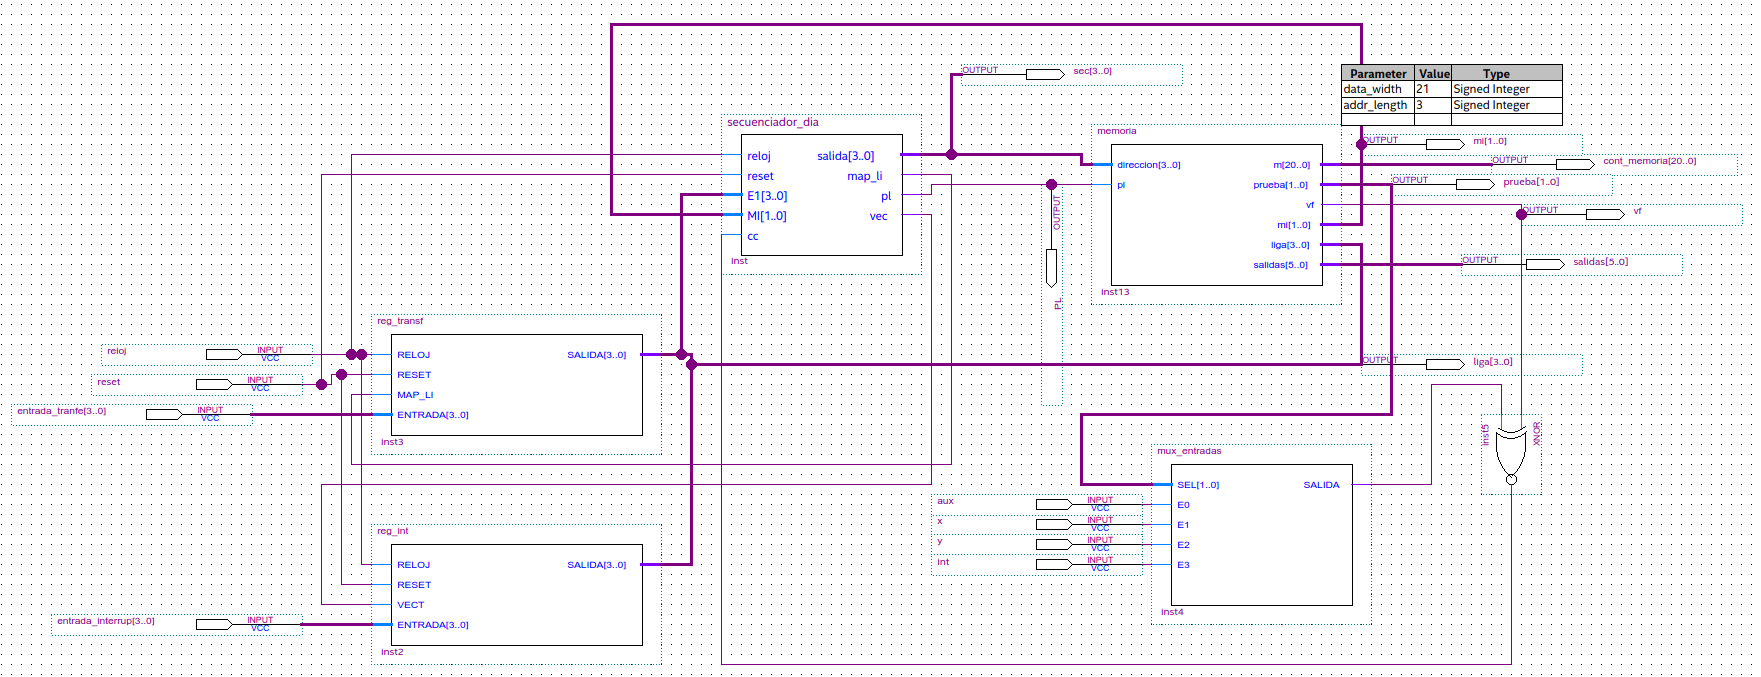
\includegraphics[width=\textwidth]{./img/fin_dia}
  \caption{Esquema del secuenciador Básico}\label{fig:fin_dia}
\end{figure}
\newpage{}
\subsection{Simulación}\label{sec:simulacion}
Simulamos varias rutas para comprobar que la implementación de la
carta ASM, probando los saltos de interrupción del estado 7 y el estado 9, y los
saltos de transferencia de transferencia del estado 4:
\begin{figure}[H]
  \centering
  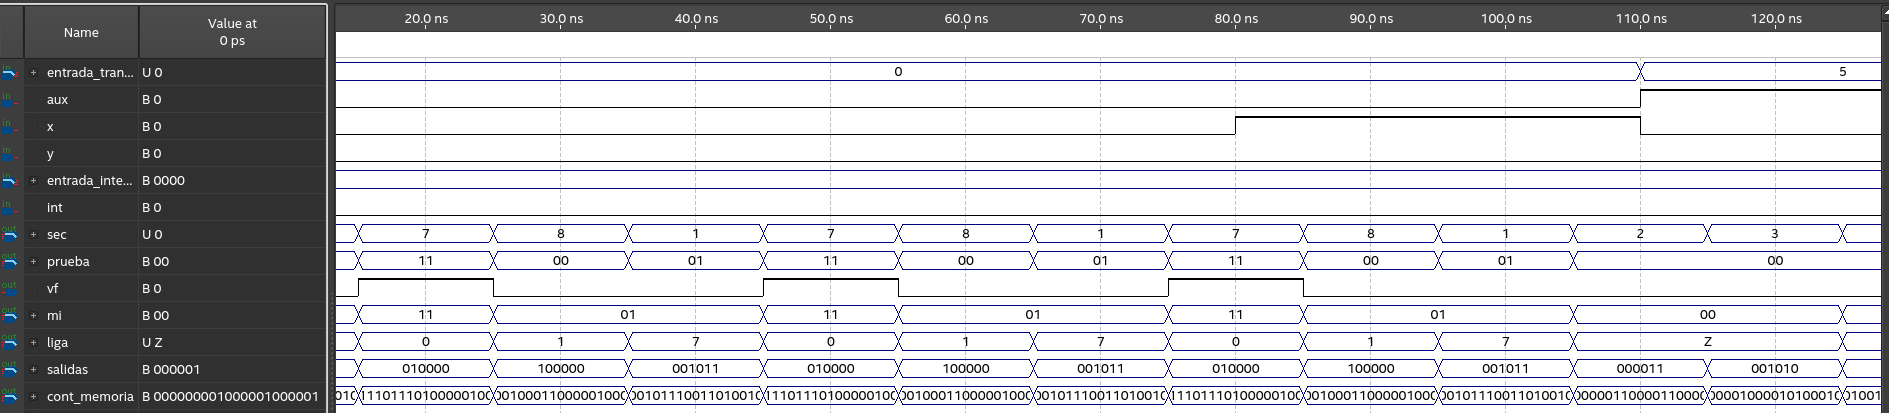
\includegraphics[width=\textwidth]{./img/sim1}
  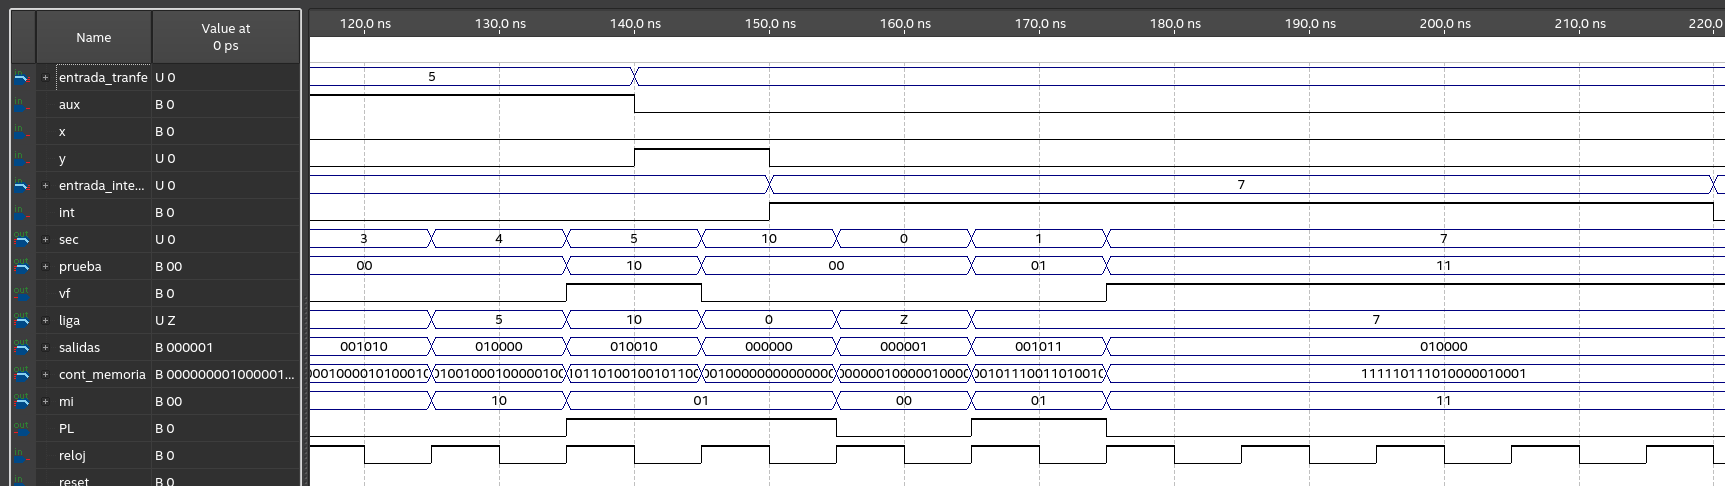
\includegraphics[width=\textwidth]{./img/sim2}\\
  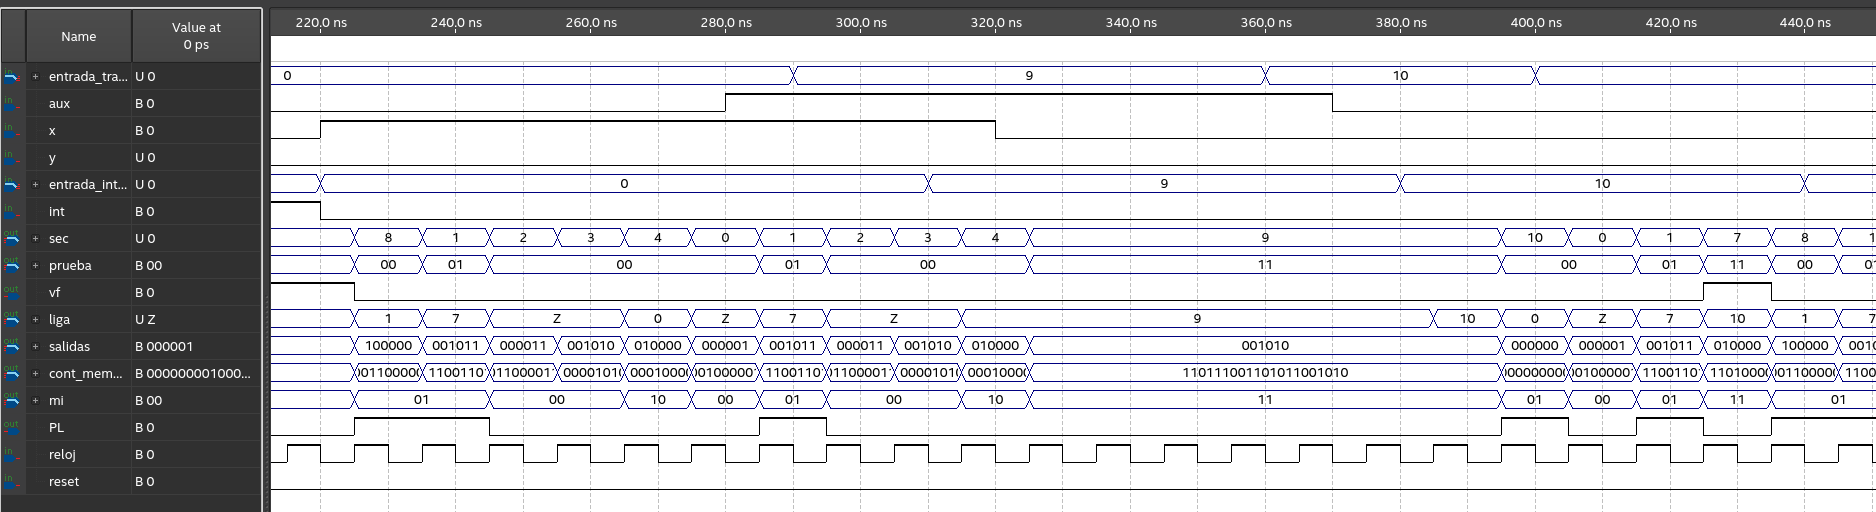
\includegraphics[width=\textwidth]{./img/sim3}\\
  \caption{Simulaciones}\label{fig:sim}
\end{figure}
\newpage{}

\section{Conclusiones}
\label{sec:conclusiones}

\paragraph{Monsalvo Bolaños Melissa Monserrat}

A través del desarrollo de esta práctica pudimos implementar un secuenciador
básico. Determinamos la lógica para la asignación del estado siguiente con base
en la micro instrucción seleccionada, activando el registro que provee el
estado, ya sea el de interrupción, el Registro de micro-programa, el registro de
transformación o la liga.

Así mismo, se decidió tomar el ```camino largo'' para el desarrollo de la práctica,
de este modo, pudimos conocer a profundidad las partes involucradas en el
desarrollo del secuenciador.

\paragraph{Romero Andrade Cristian}

Esta practica estaba dividida en dos partes, en la cual se tenia que diseñar la
lógica del secuenciador y aparte pasar y decir que acciones tomar al
secuenciador. Se implemento la carta ASM usando las MI que nosotros definimos e
implementamos para desarrollar la practica.

\nocite{*}
\addcontentsline{toc}{section}{Referencias}
\printbibliography{}


\listoftables{}
\listoffigures{}
\listoflistings{}
\end{document}
